%% V1.4b
%% 2015/08/26
%% by Michael Shell
%% See:
%% http://www.michaelshell.org/
%% for current contact information.
%%
%% Support sites:
%% http://www.michaelshell.org/tex/ieeetran/
%% http://www.ctan.org/pkg/ieeetran
%% and
%% http://www.ieee.org/

\documentclass[conference]{IEEEtran}
% Some Computer Society conferences also require the compsoc mode option,
% but others use the standard conference format.
%
% If IEEEtran.cls has not been installed into the LaTeX system files,
% manually specify the path to it like:
% \documentclass[conference]{../sty/IEEEtran}




% *** GRAPHICS RELATED PACKAGES ***
%
\ifCLASSINFOpdf
  \usepackage[pdftex]{graphicx}
  % declare the path(s) where your graphic files are
  \graphicspath{./images/}
  % and their extensions so you won't have to specify these with
  % every instance of \includegraphics
  \DeclareGraphicsExtensions{.pdf,.jpeg,.png}
\else
  % or other class option (dvipsone, dvipdf, if not using dvips). graphicx
  % will default to the driver specified in the system graphics.cfg if no
  % driver is specified.
  % \usepackage[dvips]{graphicx}
  % declare the path(s) where your graphic files are
  % \graphicspath{{../eps/}}
  % and their extensions so you won't have to specify these with
  % every instance of \includegraphics
  % \DeclareGraphicsExtensions{.eps}
\fi
% graphicx was written by David Carlisle and Sebastian Rahtz. It is
% required if you want graphics, photos, etc. graphicx.sty is already
% installed on most LaTeX systems. The latest version and documentation
% can be obtained at: 
% http://www.ctan.org/pkg/graphicx
% Another good source of documentation is "Using Imported Graphics in
% LaTeX2e" by Keith Reckdahl which can be found at:
% http://www.ctan.org/pkg/epslatex
%
% latex, and pdflatex in dvi mode, support graphics in encapsulated
% postscript (.eps) format. pdflatex in pdf mode supports graphics
% in .pdf, .jpeg, .png and .mps (metapost) formats. Users should ensure
% that all non-photo figures use a vector format (.eps, .pdf, .mps) and
% not a bitmapped formats (.jpeg, .png). The IEEE frowns on bitmapped formats
% which can result in "jaggedy"/blurry rendering of lines and letters as
% well as large increases in file sizes.
%
% You can find documentation about the pdfTeX application at:
% http://www.tug.org/applications/pdftex





% *** MATH PACKAGES ***
%
%\usepackage{amsmath}
% A popular package from the American Mathematical Society that provides
% many useful and powerful commands for dealing with mathematics.
%
% Note that the amsmath package sets \interdisplaylinepenalty to 10000
% thus preventing page breaks from occurring within multiline equations. Use:
%\interdisplaylinepenalty=2500
% after loading amsmath to restore such page breaks as IEEEtran.cls normally
% does. amsmath.sty is already installed on most LaTeX systems. The latest
% version and documentation can be obtained at:
% http://www.ctan.org/pkg/amsmath






% *** SPECIALIZED LIST PACKAGES ***
%
%\usepackage{algorithmic}
% algorithmic.sty was written by Peter Williams and Rogerio Brito.
% This package provides an algorithmic environment fo describing algorithms.
% You can use the algorithmic environment in-text or within a figure
% environment to provide for a floating algorithm. Do NOT use the algorithm
% floating environment provided by algorithm.sty (by the same authors) or
% algorithm2e.sty (by Christophe Fiorio) as the IEEE does not use dedicated
% algorithm float types and packages that provide these will not provide
% correct IEEE style captions. The latest version and documentation of
% algorithmic.sty can be obtained at:
% http://www.ctan.org/pkg/algorithms
% Also of interest may be the (relatively newer and more customizable)
% algorithmicx.sty package by Szasz Janos:
% http://www.ctan.org/pkg/algorithmicx




% *** ALIGNMENT PACKAGES ***
%
%\usepackage{array}
% Frank Mittelbach's and David Carlisle's array.sty patches and improves
% the standard LaTeX2e array and tabular environments to provide better
% appearance and additional user controls. As the default LaTeX2e table
% generation code is lacking to the point of almost being broken with
% respect to the quality of the end results, all users are strongly
% advised to use an enhanced (at the very least that provided by array.sty)
% set of table tools. array.sty is already installed on most systems. The
% latest version and documentation can be obtained at:
% http://www.ctan.org/pkg/array


% IEEEtran contains the IEEEeqnarray family of commands that can be used to
% generate multiline equations as well as matrices, tables, etc., of high
% quality.




% *** SUBFIGURE PACKAGES ***
%\ifCLASSOPTIONcompsoc
%  \usepackage[caption=false,font=normalsize,labelfont=sf,textfont=sf]{subfig}
%\else
%  \usepackage[caption=false,font=footnotesize]{subfig}
%\fi
% subfig.sty, written by Steven Douglas Cochran, is the modern replacement
% for subfigure.sty, the latter of which is no longer maintained and is
% incompatible with some LaTeX packages including fixltx2e. However,
% subfig.sty requires and automatically loads Axel Sommerfeldt's caption.sty
% which will override IEEEtran.cls' handling of captions and this will result
% in non-IEEE style figure/table captions. To prevent this problem, be sure
% and invoke subfig.sty's "caption=false" package option (available since
% subfig.sty version 1.3, 2005/06/28) as this is will preserve IEEEtran.cls
% handling of captions.
% Note that the Computer Society format requires a larger sans serif font
% than the serif footnote size font used in traditional IEEE formatting
% and thus the need to invoke different subfig.sty package options depending
% on whether compsoc mode has been enabled.
%
% The latest version and documentation of subfig.sty can be obtained at:
% http://www.ctan.org/pkg/subfig




% *** FLOAT PACKAGES ***
%
%\usepackage{fixltx2e}
% fixltx2e, the successor to the earlier fix2col.sty, was written by
% Frank Mittelbach and David Carlisle. This package corrects a few problems
% in the LaTeX2e kernel, the most notable of which is that in current
% LaTeX2e releases, the ordering of single and double column floats is not
% guaranteed to be preserved. Thus, an unpatched LaTeX2e can allow a
% single column figure to be placed prior to an earlier double column
% figure.
% Be aware that LaTeX2e kernels dated 2015 and later have fixltx2e.sty's
% corrections already built into the system in which case a warning will
% be issued if an attempt is made to load fixltx2e.sty as it is no longer
% needed.
% The latest version and documentation can be found at:
% http://www.ctan.org/pkg/fixltx2e


%\usepackage{stfloats}
% stfloats.sty was written by Sigitas Tolusis. This package gives LaTeX2e
% the ability to do double column floats at the bottom of the page as well
% as the top. (e.g., "\begin{figure*}[!b]" is not normally possible in
% LaTeX2e). It also provides a command:
%\fnbelowfloat
% to enable the placement of footnotes below bottom floats (the standard
% LaTeX2e kernel puts them above bottom floats). This is an invasive package
% which rewrites many portions of the LaTeX2e float routines. It may not work
% with other packages that modify the LaTeX2e float routines. The latest
% version and documentation can be obtained at:
% http://www.ctan.org/pkg/stfloats
% Do not use the stfloats baselinefloat ability as the IEEE does not allow
% \baselineskip to stretch. Authors submitting work to the IEEE should note
% that the IEEE rarely uses double column equations and that authors should try
% to avoid such use. Do not be tempted to use the cuted.sty or midfloat.sty
% packages (also by Sigitas Tolusis) as the IEEE does not format its papers in
% such ways.
% Do not attempt to use stfloats with fixltx2e as they are incompatible.
% Instead, use Morten Hogholm'a dblfloatfix which combines the features
% of both fixltx2e and stfloats:
%
% \usepackage{dblfloatfix}
% The latest version can be found at:
% http://www.ctan.org/pkg/dblfloatfix




% *** PDF, URL AND HYPERLINK PACKAGES ***
%
%\usepackage{url}
% url.sty was written by Donald Arseneau. It provides better support for
% handling and breaking URLs. url.sty is already installed on most LaTeX
% systems. The latest version and documentation can be obtained at:
% http://www.ctan.org/pkg/url
% Basically, \url{my_url_here}.




% *** Do not adjust lengths that control margins, column widths, etc. ***
% *** Do not use packages that alter fonts (such as pslatex).         ***
% There should be no need to do such things with IEEEtran.cls V1.6 and later.
% (Unless specifically asked to do so by the journal or conference you plan
% to submit to, of course. )


% correct bad hyphenation here
\hyphenation{op-tical net-works semi-conduc-tor}


\begin{document}

\title{INCAT : Intelligence-based Cybersecurity Awareness Training
}


% author names and affiliations
% use a multiple column layout for up to three different
% affiliations
\author{\IEEEauthorblockN{Tam Nguyen}
\IEEEauthorblockA{North Carolina State University\\
tam.nguyen@ncsu.edu - linkedin.com/in/tamcs}
}

% make the title area
\maketitle

% As a general rule, do not put math, special symbols or citations
% in the abstract
\begin{abstract}
Cybersecurity training should be adaptable to evolving cyber threat landscape, be cost effective and most important of all, be integrated well with other components such as enterprise risk management, incident management, threat intelligence and so on. Unfortunately, very few cyber security training platforms can satisfy those requirements. This paper proposes a new model for conducting cyber security trainings with three main objectives: (i) training efforts are initiated by emerging relevant threats and delivered first to respective most vulnerable members (ii) each training session must be
promptly executed (iii) training results must be able to provide actionable intelligence to be employed by other systems such as enterprise risk management, enterprise threat intelligence, etc. The model consists of a data-analytic/machine learning (DA) component and a cyber training delivery (DE) component. DE interfaces with users while DA interfaces with existing cyber security systems and/or databases. Together, DE and DA empower each other, forming a feedback loop that allow all previously-stated objectives to be met.
\end{abstract}

% no keywords




% For peer review papers, you can put extra information on the cover
% page as needed:
% \ifCLASSOPTIONpeerreview
% \begin{center} \bfseries EDICS Category: 3-BBND \end{center}
% \fi
%
% For peerreview papers, this IEEEtran command inserts a page break and
% creates the second title. It will be ignored for other modes.
\IEEEpeerreviewmaketitle

\section{Introduction}
The threat landscape is constantly changing. Something that was not considered a vulnerability yesterday may now become one \cite{Manadhata2011AnMetric}. Therefore, cyber-security awareness training (CAT) should be adaptable, be cost effective and most important of all, be integrated well with other components such as enterprise risk management, incident management, threat intelligence and so on. Unfortunately and in most cases, CAT is not a strong component in most cyber defense strategy \cite{Jakoubi2009AManagement}.

This lack of emphasis on human training and analysis leads to greater issues with establishing cyber security requirements, cyber incident's impact determination, and the simulation of possible attack scenarios. For example, security requirements tend to be mechanical 1-on-1 mappings from obvious security features and regulatory controls \cite{Cleland-Huang2014HowGratae}. Consequently, there is a very common assumption that most malicious hackers will seek the path of the most devastating exploits. In realities, hackers do not follow a straight line while using only a fraction of available vulnerabilities to deliver attacks \cite{Allodi2017TowardsAssumptions}. A lot of those vulnerabilities deal directly with human errors \cite{Messaoud2017AdvancedChallenges}.

Also, it is found that when evaluating cybersecurity risks, there are fixation on binary events without consideration of fuzzy states in between, and bias toward the point of view of security management (more technical) rather than overall business goals (more human oriented) \cite{Dhillon2011Developer-drivenTrenches} \cite{Bayuk2013SecurityConstruct}. Last but not least, common reported threat metrics can be highly debatable among teams and agencies \footnote{https://bit.ly/1yJcGjC} since numbers cannot describe all possible underlining context. 

This paper proposes InCAT - a new model for conducting cyber security training with a strong focus on drilling deep into the shared contexts among collected cyber awareness training results, cyber threat intelligence reports, and other cyber security related data logs. InCAT stands for "Intelligence-based Cyber Awareness Training" and its feedback loop starts with a threat intelligence feed where the most recent cyber threats will be analyzed by machine learning models to identify the current attack-defense themes. This angle is called "Technical Angle". From the identified themes, quizzes will be sent to users (samples) within a company (population). Machine learning models will analyze users' responses with expected results such as a list of vulnerabilities for which employees are least prepared for. This angle is called "Human Angle". Actionable intelligence can then be derived from analyzing results gathered from both angles.

The main contributions of this paper include: (i) A novel new model for conducting cyber-security awareness training that is highly adaptive to threat landscape (ii) Downloadable type system, dictionaries and human annotated data-sets for further customization and studies, (iii) Exported machine learning models and starter code base for immediate deployment. Background and related works are presented in Section 2. High-level design structure and elaborations on our methodologies are presented in Section 3. Implementation details including links to demos, source codes, sample data and results are presented in Section 4. Self-critical evaluations of this research project will be presented in Section 5 to be followed with plans for future works listed in the Conclusion section.

\section{Background and Related Works}
Human is the weakest link in any cyber defense strategy. 78\% of cyber incidents were caused by careless humans \cite{PonemonInstitute20172017Overview}. The process of cyber awareness training is full of challenges. First, the threat landscape is evolving rapidly with both internal factors (technology changes, business flows changed, etc) and external factors (changes in supply chain, compliance, competitors, enemies, political climates, etc) \cite{Ingalsbe2008ThreatEnd, Manadhata2011AnMetric}. To make things worst, there is no agile cooperation between cyber awareness education and other departments. 

Second, knowledge is not always translated into correct actions. For example, people who know the types of phishing are not completely immune from actual phishing. Training materials are more focused on teaching the knowledge rather rather the skills of applying the knowledge. Consequently, tests are developed to test just the knowledge, in which case learners are well aware that they are being tested and consciously put their guards on. It is very hard to simulate real world scenarios.

Finally, it is challenging to prepare people for potential unknown threats that have not happened yet, not mentioning cyber adversaries are incredibly creative, sometimes state sponsored. On the quest to find an effective yet affordable solution, the paper found agreements with the below-listed excellent works.

Abawajy \cite{Abawajy2014UserMethods} did a research on user preference of cyber security awareness methods of text-based, video-based and game-based among 60 participants. Even with a "low-tech" appearance, the performance of text-based education is on par with other "fancy" methods. Employees with work deadlines and projects actually prefer light-weight cyber security awareness delivery method that does not get in the way of their main jobs.

Pawlowski \cite{Pawlowski2016SocialDesign} presented a way to use data analytic to map learners' perceptions toward cyber security topics. The idea is to find out what learners care most/less, what learners are missing, and what can be leveraged to motivate learners to learn more. It was discovered that learners do have good exposures to several cyber security key terms and concepts, care very much about cyber security topics that may affect them personally, while missing a lot of the bigger picture involving national cyber infrastructure and cyber terrorism.

Wei \cite{Wei2017IntegratingAssessment} adopts concept mapping (CM) as a tool to enhance the teaching and evaluating of Information System courses. By analyzing the topology of student CMs, instructors can design CM-based tasks, and grade student CMs against a master CM. While it was not explicitly mentioned in the paper, comparing CM is a very interesting way to identify how the concept map of a student can be changed over time, by education and other factors.

Green \cite{Green2018TowardsSchemes} proposed an alternative to regular text-based machine learning approach with heavier emphasis on argument mining. The process involves steps of careful annotation of a selected corpus, building logic rules or relationships based on domain specific knowledge, and finally, inferring arguments. The paper made a case for more sophisticated content analysis method when dealing with complex contents such as biological research papers.

Joshi \cite{Joshi2013ExtractingText} described a strategy of "combining" intelligence gathered from both structured and unstructured texts to form actionable intelligence in the domain of cyber security. The approach relies on a custom ontology for cyber security domain and a "concept extractor" built using various open-source products.

Ferruci \cite{Ferrucci2010BuildingProject} wrote about IBM's billion dollar baby - Watson, and proves that within a large knowledge domain such as Jeopardy's, not only deep learning can understand human languages and response with thoughtful insights, but it can also perform reliably in real time. To sum up the strength and weaknesses of Watson, Deloitte did provide a very good report \cite{DeloitteDevelopment2015DisruptionWatson} in 2015. At the time of this paper, IBM Watson has been deployed commercially in various domains including health care, finance, insurance and so on.

\section{Methodology and Designs}
Inspired by the above-mentioned works, the paper established a few guiding principles. First, assessments can be text-based and do not have to be fancy with the uses of videos or software-based simulations. Second, context identification is crucial for situation awareness. Third, advanced and reliable AI has to be used to make sure contexts are harvested fully and correctly. Forth, the whole process has to be fast, scalable and reasonably affordable.

The InCAT design is a short and fast feedback loop, which includes 8 main steps as shown in Figure \ref{Figure:IncatDesign}. 

\begin{figure}[ht]
  \centering
  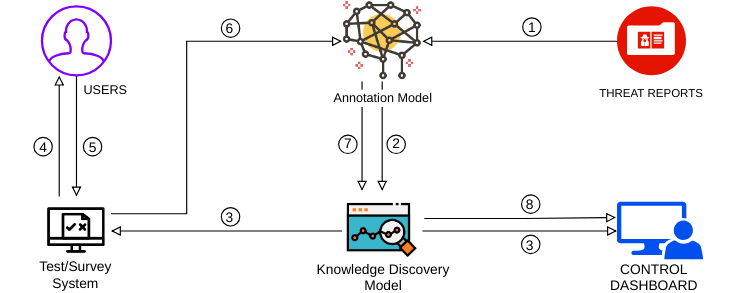
\includegraphics[width=8.8cm]{images/INCAT-Designs}
  \caption{INCAT Design Structure}
  \label{Figure:IncatDesign}
\end{figure}

Starting from step one, threat reports are highly condensed data which relate to cyber threat developments and were prepared by cyber threat intelligence experts. Reports will be analyzed by the Annotation Model for identification of key entities and their relationships. Newly annotated data will be further analyzed by the Knowledge Discovery Model which will automatically identify newly emerged patterns in cyber threat landscape. These results will be consumed by both test/survey system and the control dashboard. In step four, the Test/Survey System will construct assessments based on the knowledge components relating to the newly identified patterns and deliver to the users who are most vulnerable. Assessment results will then be returned to the Test/Survey System for initial processing, resulting in two products: reports with scores and structured text-based feedback strings. Feedback strings will be analyzed by the same Annotation Model and the Knowledge Discovery Model. Derived knowledge from threat reports (step 3) and feedback strings (step 7) are stored in database to be displayed or analyzed at any later time. Through the control dashboard, InCat system administrators may manually correlate details and derive further actionable intelligence.

\subsection{The Test-Case Design}
In order to find more meaningful contexts between the technical angle and the human angle, test-cases must be generated. Each test case should have only one investigation interest. For example, the potential number of employees who may be tricked into launching a certain type of malicious app on Android play store. Each test case has a database of entries each of which has a format as followed.

\subsubsection{The User Assessment Result Section}
This section is mandatory for each entry within the Test-case database and is constructed by users' responses to past cyber security knowledge assessments. Ideally, for each test case, a round of assessment quizzes/surveys should be sent out to potentially most vulnerable employees using combined intelligence from system usage logs, cyber threat reports, previous survey results, and so on.

Each response to a survey question will be recorded as a group of maximum three entities (keywords) and a status word ("Passed" or "Failed"). The entities describe the cyber security scenario being tested by the question and such entities follow the InCAT system type to be discussed in later section. The survey designer when designing an assessment will hand-code those entities in. An example of one recorded user response could be "Passed: MS Windows, MS Word, Malicious attachment".

It is important to note that a well-designed cyber security question must not be straight forward and should involve several related knowledge components in order to mimic the complexity of real-world situations. By mapping the question's contents into those entities, we allow machine models to "read" all different types of survey questions, some of which may involve pictures and videos.

\subsubsection{The Entity Pair Section}
This section is optional providing the Random Concept Section exists. Highly relevant entities are grouped in pairs and the section may have up to two pairs. For example, "Android phone, mobile banking" is a good pair while "Android phone, ATM machine" is not. These pairs may be the results of analyzing cyber threat reports, analyzing a group of employees' digital behaviors, or any data source other than user cyber-security assessment database.

The main purpose of paring up entities in this section is about inferring indirect impacts. For example, if there are evidences of serious knowledge gaps in safe use of Android Operating System, it will be reasonable to assume the users will also be vulnerable to mobile banking hacks.

\subsubsection{The Random Entity Section}
This section is optional providing the Entity Pair Section exists. Up to three entities that are independent from each other can be present. For example, we may have "Windows, iPhone, ATM machines". Such structure is fit for describing loosely connected knowledge domains such as the cyber security knowledge of a new employee, top 3 categories of user reported IT issues, etc.

While this section appears to be inferior to the Entity Pair Section, it is more realistic and remains more objective. In some cases, there might be hidden links between seemingly "disconnected" entities. In other cases, cyber attacks may target totally unrelated entities because those attacks are from different groups of bad actors.

In short, each section represents associated topics from a certain domain. The User Assessment Result section represents users' knowledge domain while other sections may represent threat landscape domain, operational business domain, etc. The content of each entry in a test case will be analyzed by a Natural Language Processing (NLP) model - the annotation model - in order to find out "links" among entities across domains. These "links" or "basic relationships" form the foundation for more complex contextual-based queries performed by the Knowledge Discovery Model.


\subsection{The Type System}
There are three main steps for building the Annotation Model: (i) Building a system type (ii) Building ground truths by careful manual annotation (iii) Training and evaluating models.

A system type is a domain-specific ontology enriched with relationships. The ontology serves as the core of a common language describing cyber security vulnerabilities that all models within the InCAT system will use. A well-designed ontology is crucial in finding actionable intelligence across domains, in highly complicated situations such as court cases \cite{Michel2018CyberCybercrime}. However, there are at least two big problems with existing cyber security ontologies: incomplete and incompatible \cite{Mavroeidis2017CyberIntelligence}. We decided to rely on the NIST's recommendations for Cyber Vulnerability Description ontology \cite{Booth2016DraftOntology} which we summarized into Figure \ref{Figure:VulOntology}. While being not perfect, NIST's ontology for Cyber Vulnerability Description appears to be the latest attempt with continuing development efforts sponsored by the US Government.

\begin{figure*}[ht]
  \centering
  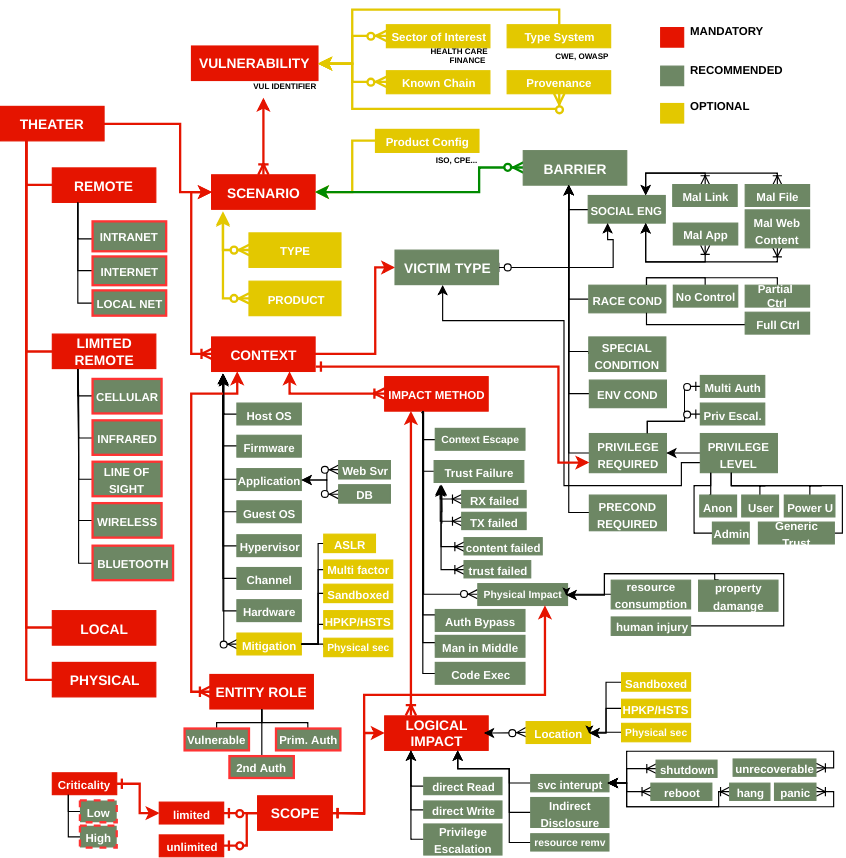
\includegraphics[width=16cm]{./images/NISTIR8138}
  \caption{Vulnerability Description Ontology}
  \label{Figure:VulOntology}
\end{figure*}

It is notable that in real-world scenario, reports will only touch a few "boxes" of this crowded ontology. Therefore, the ontology has to be enriched with relationships that are context-preserving. Such relationships can be described directly by rules or indirectly by type \& sub-type specifications. The novelty of this paper comes in the form of its own designed relationship rules, the overloading of the rules and the re-mapped hierarchy of the original NIST's ontology.

More specifically, "Type and sub-types" structure will be applied to parent who can only have one child among a list of options. "Narrow" relationships are the ones that have only one type at one end and only one type at another end (A relates-to B). "Wide" relationships are the ones that have multiple types at either or both ends ( a set of {A,B,C} relates-to a set of {D,E,F} ). The relationships between keywords found in paragraphs can be overloaded by two ways. An entity (keyword) can play the role of its corresponding type or the role of its parent. An entity (keyword) can be marked with two types.

For example, "4G mobile network" can play the role of "Cellular" under "Theater" or it can be assigned the role "Theater" itself. We recall that narrow relationship requires a particular type and if there is no other entity to play the role of "Theater", "4G mobile network" should be able to step up and play that role. It can also play the "Celular" type and another type such as "Channel" under "Context". We note that "role" is used among members of the same type (parent and its sub-trees) while types refers to members of different branches.

The detailed description file of the type system (ontology with relationships) can be viewed at the project's Github repository \footnote{https://github.com/genterist/INCAT-public}.

\subsection{The AI/Machine learning process}
The process contains cycles of: pre-annotation, manual annotation, training, and evaluating. In the absence of a previously built model, pre-annotation can be performed based on dictionaries. Key entities will be labeled and then domain experts will annotate the rest manually. The manual annotation makes sure correct types are assigned and the relationships between identified entities are full and accurate. Different domain experts will annotate different sets with a certain amount of overlapping. Manually annotated results will be analyzed by "referees" who will take a look into conflicting results and make the final decisions.

Ground-truths are manually annotated sets that were approved by referees. Based on these ground-truths, the training set, the testing set and the blind set will be formed. Following regular machine learning training practices, the training process will be separated into rounds. Each round has its own randomly selected training set and testing set from ground truths. Blind set contains items that do not belong to any training or testing set.

Accuracy is calculated based on both testing set and blind set. In each round, after round model was trained with the training set, the model will analyze the testing set and produce its own results. These results will be compared with human annotated results (ground truths) associated with items in the testing set. A percentage reflects how well the machine produced results match the human annotated results. After certain rounds, the best model with the highest percentage will be selected. This model will then analyze the blind set, compare results and adjust the accuracy (the percentage) for one last time.

\section{Implementation and Results}
The project employs IBM Cloud and IBM Watson system and at this moment, the results include: (a) A good Type System with 12 dictionaries, 38 entity types and 66 relationship types; (b) A good annotated corpus with 100 threat reports (manually annotated), 127 knowledge assessment results (manually annotated), and 8000 threat reports (automatically annotated). All of these results are available for downloading at the project's GitHub repo \footnote{https://github.com/genterist/INCAT-public}.

\subsection{Designing Cyber Security Knowledge Assessment}

\begin{figure}[ht]
  \centering
  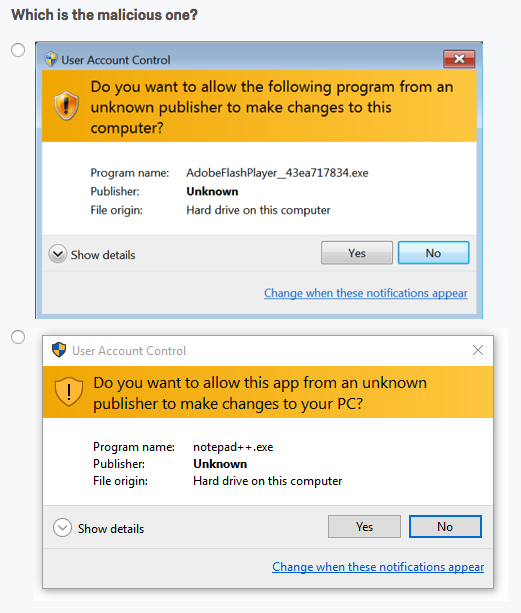
\includegraphics[width=8cm]{images/quiz-sample}
  \caption{Quiz sample}
  \label{Figure:quiz-sample}
\end{figure}

lorem ipsum

\begin{table}[]
\begin{tabular}{|l|c|}
\hline
{}&{} \\[-0.5em] 
{\textbf{TESTED KNOWLEDGE} } & \textbf{FAILED RATE} \\[2pt] \hline
& \\[-0.8em] 
Malicious Windows file                          & 63\%                 \\[2pt] \hline
{}&{} \\[-0.8em] 
Malicious Android app                           & 34\%                 \\[2pt] \hline
{}&{} \\[-0.8em] 
Online MS Office scam                           & 41\%                 \\[2pt] \hline
{}&{} \\[-0.8em] 
Fake web pages                                  & 12\%                 \\[2pt] \hline
{}&{} \\[-0.8em] 
Effects of ransomwarez                          & 23\%                 \\[2pt] \hline
{}&{} \\[-0.8em] 
Desktop MS Office scam                          & 35\%                 \\[2pt] \hline
\end{tabular}
\end{table}

\subsection{Annotating Feedback Strings}
The Knowledge Discovery Model is an analytic engine with a front end and a back end. The front end (the Control Dashboard) displays identified patterns, trends and actionable insights using Node.js, React, Semantic UI React, and Chart.js. The back end accepts inputs produced by the annotation model, communicates with IBM Watson Discovery Service API, and renders the views that will be displayed on the front end. The server will also communicate with Qualtrics API in order to initiate the delivery of tests (surveys) to users. The user knowledge testing components will be discussed further in our full paper.

\begin{figure*}[ht]
  \centering
  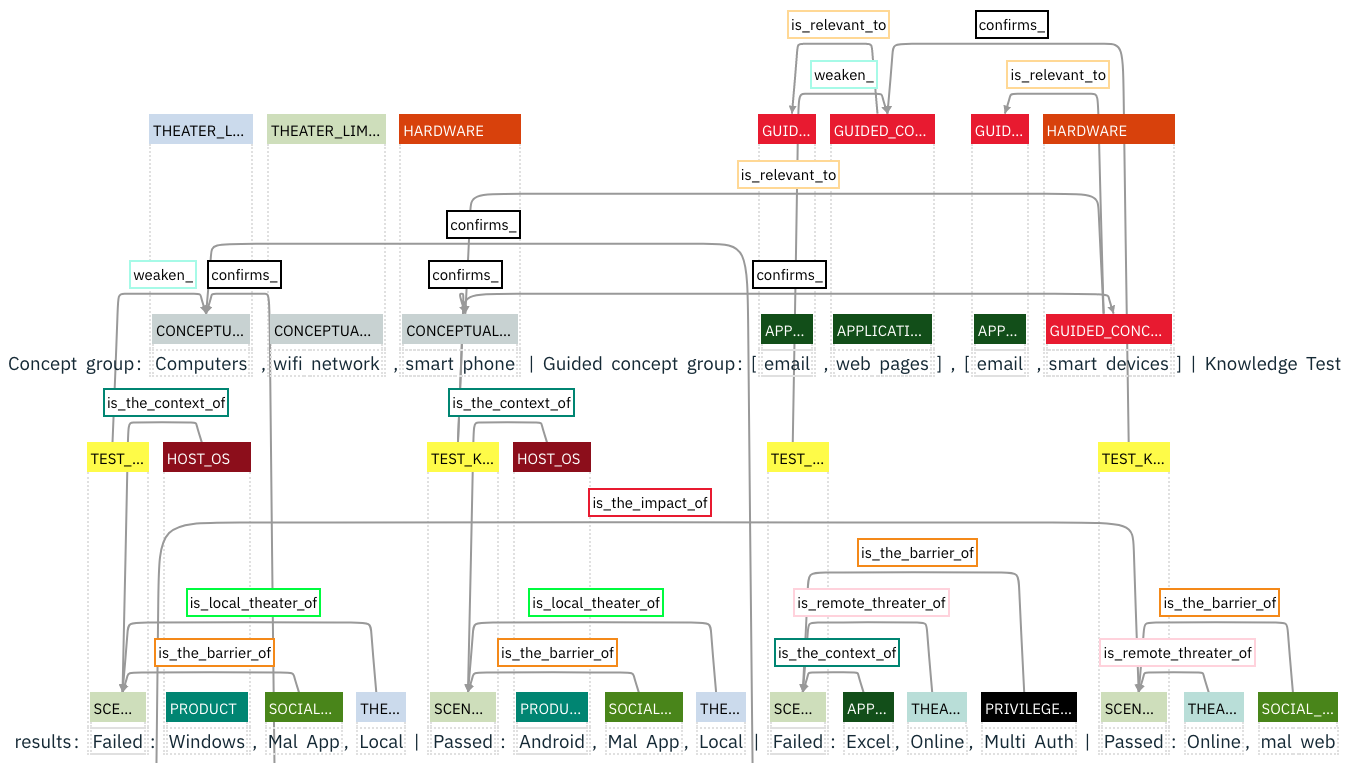
\includegraphics[width=16cm]{./images/feedbackString}
  \caption{Feedback String Annotation}
  \label{Figure:feedbackString}
\end{figure*}

\subsection{Annotating Cyber Threat Reports} 
Categorical data from National Vulnerability Database \footnote{https://nvd.nist.gov/vuln} was used to create a hierarchical cluster that would serve to inform the annotation and classification process used in 4.2 and provide the underlying framework for the identification and selection of Attack Vectors. The project's data-sets of Threat Reports were extracted from the National Vulnerability Database that is being used nation wide. In the form of XML or CSV files, data-sets can be imported into Annotation Model which is powered by the IBM Watson Knowledge Studio platform \footnote{https://www.ibm.com/watson/services/knowledge-studio/}.

In order to build ground truths, we started first with human annotators and manual annotation. Small sets of 50 entries each are extracted from our corpus of 1000 NVD threat reports in 2018. Sets can be specified to have some overlaps in order to support inter-annotation. Team members (except one) will work on their corresponding pre-assigned sets and manually annotate entities together with relationships. At the final step, the one who did not do any manual annotation will go over the results, resolve conflicts and publish annotated entries as ground truths.

On the IBM Watson Knowledge Studio platform, we train and test our models using the manually annotated entries which are separated into training set (70\%), test set(23\%), and blind set(7\%). Training set is used to teach machine the domain specific knowledge through annotated entities and their relationships. Trained model will then perform on test set to produce test set machine results. Upon comparing test set machine results with human annotated results, the accuracy of the model can be defined. Blind set is used to test the system only after several iterations of training and testing. The end result of this process is an annotation model that can be deployed with other models which, in our case, happened to be IBM Knowledge Discovery.

\subsection{Training Annotation Model}
lorem ipsum

\begin{figure*}[ht]
  \centering
  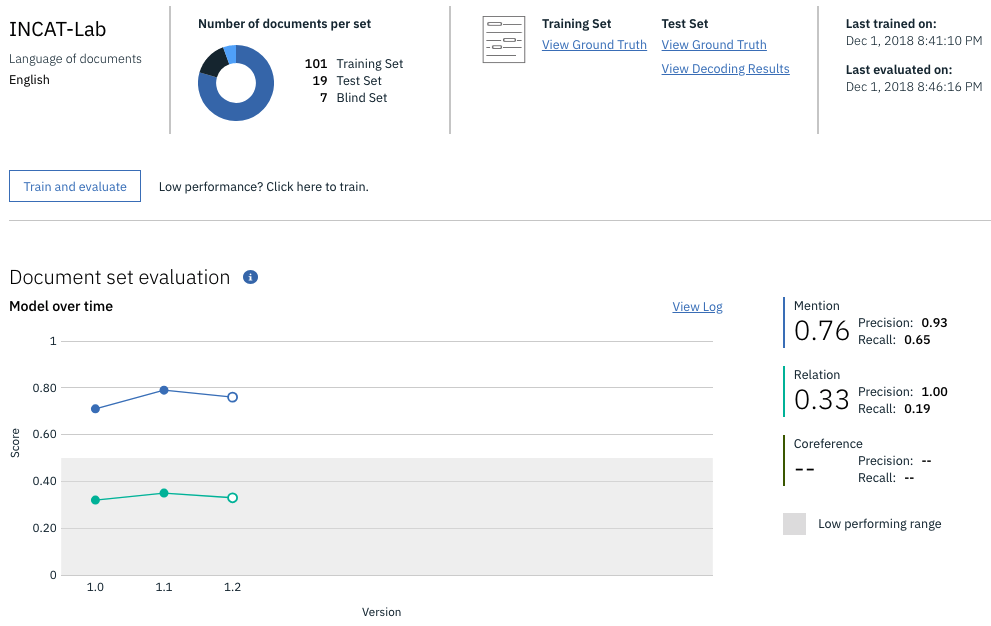
\includegraphics[width=14cm]{./images/trainingResults}
  \caption{Training results}
  \label{Figure:trainingResults}
\end{figure*}

\section{Analysis}
At the moment, we have a corpus of over 8000 cyber vulnerability report for 2018 harvested from the National Vulnerability Database (NVD) and 127 user survey entries gathered from a Qualltric-MechanicalTurk campaign. We established a type system and manually annotated 100 entries of NVD corpus and 27 entries of the user survey corpus. It will be slow in the beginning because members who do not have solid backgrounds in cyber security will need more time to annotate cyber threat reports. We are, however, in the process of making over 20 dictionaries covering main entities in our established type system so that in the next few days, machine can help us annotate the key terms in the reports.

A basic dashboard is being built utilizing IBM Watson Knowledge Discovery on top of Watson Knowledge Studio. The near term goals include counting and displaying the counts of relationship types inferred by the AI and ML models. Ultimately, we would like to be able to display inferred statistics from the cyber threat report angle and the user knowledge angle. Please note that these "statistics" are the results of machine models reading and understanding the hidden context behind cyber threat reports and survey takers responses.

\section{Conclusion}

InCAT - a new model for conducting cyber security training with three long term goals: (i) training efforts are initiated by emerging relevant threats and delivered first to the most vulnerable groups (ii) each training session must be promptly executed (iii) training results must be able to provide actionable intelligence to be employed by other systems such as enterprise risk management, enterprise threat intelligence, etc.

Our team believes we are on the right schedule to a conference quality paper. We will do further researches to make sure our existing type system is a good one, our human annotated corpus are of high quality with the right quantity, and a good Github repo with carefully documented source codes and data.Due to issues with Overleaf, we had to submit the paper in the state that you have seen. A more detailed, polished version will be readied by appropriate deadline.

% An example of a floating figure using the graphicx package.
% Note that \label must occur AFTER (or within) \caption.
% For figures, \caption should occur after the \includegraphics.
% Note that IEEEtran v1.7 and later has special internal code that
% is designed to preserve the operation of \label within \caption
% even when the captionsoff option is in effect. However, because
% of issues like this, it may be the safest practice to put all your
% \label just after \caption rather than within \caption{}.
%+
% Reminder: the "draftcls" or "draftclsnofoot", not "draft", class
% option should be used if it is desired that the figures are to be
% displayed while in draft mode.
%
%\begin{figure}[!t]
%\centering
%\includegraphics[width=2.5in]{myfigure}
% where an .eps filename suffix will be assumed under latex, 
% and a .pdf suffix will be assumed for pdflatex; or what has been declared
% via \DeclareGraphicsExtensions.
%\caption{Simulation results for the network.}
%\label{fig_sim}
%\end{figure}

% Note that the IEEE typically puts floats only at the top, even when this
% results in a large percentage of a column being occupied by floats.

% An example of a double column floating figure using two subfigures.
% (The subfig.sty package must be loaded for this to work.)
% The subfigure \label commands are set within each subfloat command,
% and the \label for the overall figure must come after \caption.
% \hfil is used as a separator to get equal spacing.
% Watch out that the combined width of all the subfigures on a 
% line do not exceed the text width or a line break will occur.
%
%\begin{figure*}[!t]
%\centering
%\subfloat[Case I]{\includegraphics[width=2.5in]{box}%
%\label{fig_first_case}}
%\hfil
%\subfloat[Case II]{\includegraphics[width=2.5in]{box}%
%\label{fig_second_case}}
%\caption{Simulation results for the network.}
%\label{fig_sim}
%\end{figure*}
%
% Note that often IEEE papers with subfigures do not employ subfigure
% captions (using the optional argument to \subfloat[]), but instead will
% reference/describe all of them (a), (b), etc., within the main caption.
% Be aware that for subfig.sty to generate the (a), (b), etc., subfigure
% labels, the optional argument to \subfloat must be present. If a
% subcaption is not desired, just leave its contents blank,
% e.g., \subfloat[].


% An example of a floating table. Note that, for IEEE style tables, the
% \caption command should come BEFORE the table and, given that table
% captions serve much like titles, are usually capitalized except for words
% such as a, an, and, as, at, but, by, for, in, nor, of, on, or, the, to
% and up, which are usually not capitalized unless they are the first or
% last word of the caption. Table text will default to \footnotesize as
% the IEEE normally uses this smaller font for tables.
% The \label must come after \caption as always.
%
%\begin{table}[!t]
%% increase table row spacing, adjust to taste
%\renewcommand{\arraystretch}{1.3}
% if using array.sty, it might be a good idea to tweak the value of
% \extrarowheight as needed to properly center the text within the cells
%\caption{An Example of a Table}
%\label{table_example}
%\centering
%% Some packages, such as MDW tools, offer better commands for making tables
%% than the plain LaTeX2e tabular which is used here.
%\begin{tabular}{|c||c|}
%\hline
%One & Two\\
%\hline
%Three & Four\\
%\hline
%\end{tabular}
%\end{table}


% Note that the IEEE does not put floats in the very first column
% - or typically anywhere on the first page for that matter. Also,
% in-text middle ("here") positioning is typically not used, but it
% is allowed and encouraged for Computer Society conferences (but
% not Computer Society journals). Most IEEE journals/conferences use
% top floats exclusively. 
% Note that, LaTeX2e, unlike IEEE journals/conferences, places
% footnotes above bottom floats. This can be corrected via the
% \fnbelowfloat command of the stfloats package.





% references section

% can use a bibliography generated by BibTeX as a .bbl file
% BibTeX documentation can be easily obtained at:
% http://mirror.ctan.org/biblio/bibtex/contrib/doc/
% The IEEEtran BibTeX style support page is at:
% http://www.michaelshell.org/tex/ieeetran/bibtex/
%\bibliographystyle{IEEEtran}
% argument is your BibTeX string definitions and bibliography database(s)
\bibliographystyle{IEEEtran}
\bibliography{IEEEabrv,references.bib}
%
% <OR> manually copy in the resultant .bbl file
% set second argument of \begin to the number of references
% (used to reserve space for the reference number labels box)
\def\url#1{}

% that's all folks
\end{document}


